\vspace*{1pc}

Cosmology, the \textit{Logos} or inquiry into the world, is by no means a recent endeavor. What I describe in this section is our current interpretation of the \textit{Cosmos} we inhabit. The basic axioms that we rely on are that \\
\begin{itemize}
\item[$\bullet$] the cosmological principle, \textit{i.e.} the Universe is spatially homogenous and there are no special reference frames or observers\footnote{known as the Copernican Principle}, and
\item[$\bullet$] general relativity is the correct description of gravity, and \\
\end{itemize} The former is observationally motivated, and it has been proven that the distribution of matter is \emph{statistically} homogenous and isotropic to within $10^{-5}$ on large enough scales, \textit{i.e.} beyond a few Gpc\footnote{$1~\mathrm{Gpc} = 10^3~\mathrm{Mpc}$, where a Mpc is the typical physical distance between two galaxies.}. Several missing pieces make our interpretation incomplete, however, since general relativity isn't predictive at the singularity of black holes, and because of observational oddities such as dark energy, the horizon problem \textit{etc}. Our current incomplete picture rests on the observation that the Universe is in a perpetual expansion state. In this section, I describe the general relativity framework in which this observation is interpreted.

\subsection{The Geometry of Spacetime}

It is arguably during the 1930's that \emph{modern} cosmology was born. Following Vesto Slipher's and Edwin Hubble's discovery of extra-galactic nebul{\ae} --- which many turned out to be entire galaxies in their own right --- it was apparent that the Universe was not a static system. The consistent redshifting of these objects' light with their distance from us, regardless of where they are in the sky, was evidence that the Universe was expanding in a homogenous and isotropic manner, owing to the observation that there seemed to be no center from which the expansion was occuring and that the expansion was similar in any direction one looked. Making sense of this startling observation in the framework of the freshly developped general relativity required introducing a particular system of coordinates that is unchanging with this expansion.
One can write the physical coordinate of an object as $x(t) = a(t) \chi$ with $a$ the scale factor and $\chi$ the (time independant) coordinate of that object in that \emph{comoving} system.
Because of homogeneity, the scale factor is homogenous in space: $a(\vec{x}, t) = a(t)$. The physical velocity can be expanded into two terms:
\begin{equation}
\label{eq:hubble_flow}
\begin{array}{cl}
\cfrac{d x}{d t} &= \cfrac{d a }{d t} \chi + a(t) \cfrac{d\chi}{dt}\\
&=\cfrac{1}{a}\cfrac{da}{dt} x + a \dot{\chi}\\
&= H x + v_{\mathrm{pec}}
\end{array}
\end{equation} \\ where the right-most term is the galaxy's peculiar velocity, \textit{i.e.} its velocity with respect to the comoving coordinate system. The left-hand term is known as the Hubble flow. The (logarithmic) rate of change in the scale factor is known as the \textbf{expansion rate}, also known as the Hubble function:
\begin{empheq}[box=\mymath]{equation}
\label{def:Hubble}
H = \frac{1}{a} \frac{da}{dt}
\end{empheq}


\subsubsection{The Fabric of Spacetime}

The isotropic and homogeneous characteristics of the expansion implies, from a mathematical point of view, that only 2 parameters fully determine the geometry of the Universe: the scale factor $a$ which can only be a (undetermined) function of time because of homogeneity and a global curvature parameter $\kappa$ which must be constant because of isotropy. The geometry on any vector space including the 4-dimensional spacetime of relativistic physics is determined by the dot product $\pmb{g}$. It is the bilinear, non-degenerate symmetric form that verifies \\

\begin{eqnarray}
\pmb{g}: ~~ \begin{array}{ccc}
\mathbb{R}^n \times \mathbb{R}^n & \longrightarrow &\mathbb{R}\\
\left( \vec{u}, \vec{v} \right) & \longmapsto & \vec{u} \cdot \vec{v} = \displaystyle \sum_{i=1}^{n}\sum_{i=1}^{n}~g_{ij} u^i v^j
\end{array}
\end{eqnarray} \\

The form $\pmb{g}$ is bilinear in $\vec{u}$ and $\vec{v}$ and so defines a tensor, called the metric tensor on $\mathbb{R}^n$, or \textbf{metric} for short. Its components\footnote{see Appendix~\ref{apx:tensors}} $g_{\mu \nu}$ are the dot product of the basis vectors $\left( \hat{e}_1, \hat{e}_2, \hdots, \hat{e}_n \right)$ in which $\vec{u}$ and $\vec{v}$ are expressed:
\begin{equation}
g_{ij} \doteq \pmb{g} \left( \hat{e}_i, \hat{e}_j \right)
\end{equation} In Euclidian space, it is always possible to define a unitary orthogonal basis. In this basis, the components of the metric are therefore the Kronecker symbol because of the orthonormalisation identities: $\hat{e}_i \cdot \hat{e}_j = \delta_{ij}$. Because $\pmb{g}$ is non-degenerate, the inverse metric exists and its contravariant components verify $g^{i k} g_{k j} = \delta^i_j$ where I use the conventional implicit summation over repeated indices. In relativity, the time component is incorporated along with the spatial coordinates in a 4-vector: $\pmb{X} = (-ct, \vec{x})$, such that the path of any free-falling massless particle has a null 4-position: $\pmb{X}^2 = 0$, which is another way of expressing $r = ct$ where $r^2 = x^2 + y^2 + z^2$. The dot product is always implicitly performed with respect to the metric. Given the minus sign in the definition of 4-vectors, the components of the metric tensor in relativity are the Minkowski symbol ($\neq$ Kronecker): \\

\begin{equation}
\label{eq:Minkowski}
g_{\mu \nu} \doteq \hat{e}_{\mu} \cdot \hat{e}_{\nu} = \eta_{\mu \nu} = \left\{ 
\begin{array}{rl}
-1 & \text{if}~\mu = \nu = 0\\
1 & \text{if}~\mu = \nu \neq 0\\
0 & \text{if}~\mu \neq \nu\\
\end{array}
\right. = \left(
\begin{array}{rccc}
-1 & 0 & 0 & 0\\
0 & 1 & 0 & 0\\
0 & 0 & 1 & 0\\
0 & 0 & 0 & 1
\end{array}
\right)
\end{equation} \\ The negative time component signature apparent in expression~\ref{eq:Minkowski} shows that spacetime is non-Euclidian contrary to $\mathbb{R}^3$ in classical physics. The dot-product is \emph{not} defined positive in relativity since vectors can have negative 4-distance $ds^2 = g_{\mu \nu}dx^\mu dx^\nu$. I am using the convention of labelling the indices with greek letters ($\mu, \nu, \alpha, \beta$). Notice the $\mu=0$ component for time is expressed in units of $c$ such that the orthogonal basis is unitary. In the framework of cosmology, it is generally more useful to adopt the opposite convention with respect to general relativity: with the time component being a positive quantity such that time-like worldlines, \textit{i.e.} curves in spacetime linking two causally connected events, are seperated by a positive distance. \\

\subsubsection{The Robertson Walker metric}

As stated, there is always a system of coordinates in which the components of the metric tensor can be expressed as Eq.~\ref{eq:Minkowski}, at the sacrifice of allowing the coordinate system to \emph{not} pertain to an inertial frame of reference. In a Universe that expands uniformly in all directions, one can find such a \emph{comoving} coordinate system, introduced at the start of this section. Objects moving apart in the Hubble flow (left term of expression \ref{eq:hubble_flow}) are at rest in this comoving coordinate system ($v_{\mathrm{pec}}=0$). The elemental distance $d\ell$ in the 3-dimensional hypersurfaces of spacetime (the purely spatial components of events, labelled by latin indices $i, j, k$) can be expressed in spherical coordinates centered on an observer:
\begin{equation}
\label{def:dell}
d\ell^2 = \frac{dr^2}{1-\kappa r^2} + r^2 d\Omega^2
\end{equation} \\ where $d\Omega^2 = d\theta^2 + \sin^2 \theta ~d\varphi^2$ is the elemental solid angle. The spherical coordinate system centered on an observer is a natural choice in an isotropic Universe, which we assume here in addition to the Copernican (or ergodic) principle, which states that there is no special observer. Both of these conditions, known as the \emph{cosmological principle}, assures spatial homogeneity. From here onwards, I use spatial homogeneity and isotropy  interchangeably with the cosmological principle, even thought the former is a statement about the global geometry of spacetime while the latter is its observational consequence. Since the vector propagating time intervals is perpandicular to all three spatial directions: $\hat{e}_0 \cdot \hat{e}_i = 0$, we can consider spatially homogenous and isotropic hypersurfaces perpandicular to time which have constant global curvature. Because of isotropy, it is possible to rescale the constant curvature parameter $\kappa$ such that \\
\begin{equation}
\kappa = \left\{
\begin{array}{rl}
+1 & \text{for positively-curved space, like 3-spheres}~ \mathbb{S}^3\\
0 & \text{for flat space, like Euclidian}~ \mathbb{R}^3\\
-1 & \text{for negatively-curved space, like 3-hyperboloidal saddles}~ \mathbb{H}^3
\end{array}
\right.
\end{equation} \\
In the first, second and third case respectively, triangles defined between three points have angles that sum to more, exactly and less than $\pi$ radians, and the circumference of a circle is more, exactly or less than $\pi$ in units of its diameter (see Fig.~\ref{fig:geocurv}). \\

\begin{figure}
\begin{center}
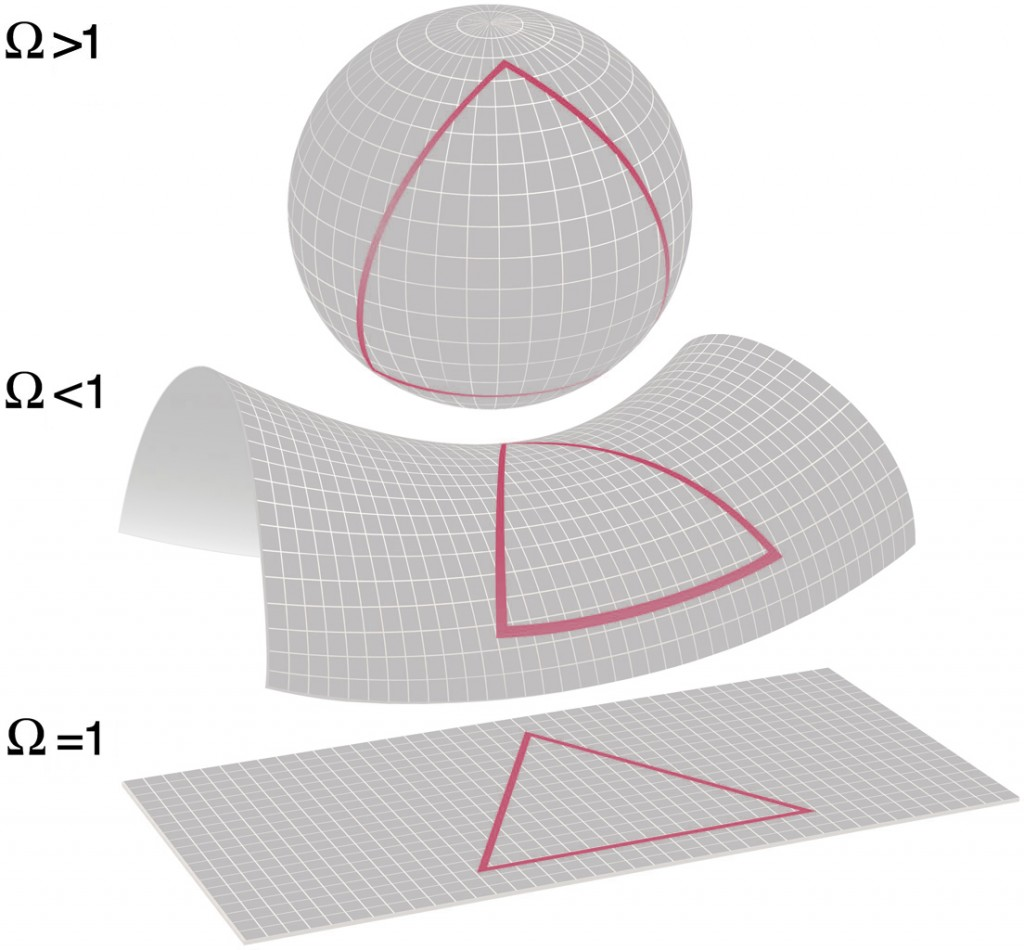
\includegraphics[width=0.75\columnwidth]{Cosmology/Big-Bang-shape.jpg}
\caption{The three categories of global geometry of a 2-dimensional Universe embedded in a 3-dimensional manifold. The critical density in its own units $\Omega$ is defined in expression~\ref{def:omega}. Credit: NASA/Hubble, public domain.}
\label{fig:geocurv}
\end{center}
\end{figure}


The simplest metric describing the geometry in a homogenous and isotropic expanding (or contracting !) Universe is the Robertson Walker metric, \textit{a.k.a.} the Friedmann Robertson Walker (FRW) metric. The line element is\\

\begin{equation}
\label{eq:RWmetric}
ds^2 = a^2 (\tau) \times \left( d\tau^2 - d\ell^2 \right)
\end{equation} \\ where the scale factor is factored out to define a \emph{conformal time} interval $d\tau = dt/a(t)$ which is the amount of time elapsed in between two events separated by a comoving elemental distance\\

\begin{equation}
d\chi = \frac{dr}{\sqrt{1 - \kappa r^2}}
\end{equation} \\ Depending on the global constant curvature of the Universe, the radial and comoving coordinates are linked by\\

\begin{equation}
\label{eq:RWmetric_space}
d\ell^2 = \gamma_{ij} dx^i dx^j = d\chi^2 + S^2_{\kappa} (\chi) d\Omega^2
\end{equation} \\ where $S_{+1, 0, -1} (\chi) = (\sin \chi, \chi, \sinh \chi)$ and $\pmb{\gamma}$ is the metric restricted to spatial coordinates only. 


\subsection{Motion Through Spacetime}

I've described the geometry of the Universe, which is useful in measuring distances between objects. The dynamics of objects in the Universe is all embeded in the FRW metric, and depends on whether the object of study is relativistic or not, which I lay out in this subsection.

\subsubsection{Equations of Motion}

Newton's principle of inertia states that an object's velocity is constant in an inertial frame of reference unless acted upon by a force, in which case the amplitude of the force equals the rate of change in the object's momentum. In the absence of any exterior interactions, the principle of inertia yields the conservation of kinetic energy $p^2 / 2m$ where $\vec{p}$ is the particle's linear momentum, which can be written as \\

\begin{equation}
\label{eq:kinetic}
\frac{\partial}{\partial t} \left( \frac{p^2}{2m} \right) = \vec{0} = \vec{p} ~ \frac{\partial}{\partial t} \vec{p}
\end{equation} \\

In general relativity, the motion of an object through curved (non-flat) space rids of the notion of a gravitational force. Gravity is essentially a property that emerges from different reference frames in a non-uniform metric. To get the equivalent of the point particle's mass and its equation of motion, we must define two quantities which are intrinsically defined on the particle's world line and do not depend on any observer (not everything is relative in relativity !). Given its 4-position $\pmb{X} = (x^0, \vec{x})$, the particle's 4-velocity and 4-momentum are respectively defined as:
\begin{align}
\pmb{U} &\doteq \frac{1}{c} \frac{d \pmb{X}}{dt}\\
\pmb{P} &\doteq m \frac{d \pmb{X}}{dt} = \left( \frac{E}{c}, \vec{p} \right)
\end{align} where $E$ is the total energy and $dt$ is the particle's \emph{proper time} defined as $c^2 dt^2 = ds^2$. These expressions introduce the particle's \emph{rest mass}, $m \geq 0$, as defined in the framework of general relativity, again an intrinsic property independant of any observer. Notice that the 4-velocity is defined as unitary, and so it follows that
\begin{align}
\label{eq:4velocity}
&\pmb{U} \cdot \pmb{U} = 1
&\pmb{P} \cdot \pmb{P} = m^2 c^2
\end{align} Photons obey $\pmb{P} \cdot \pmb{P} = 0$ and hence are massless\footnote{but they have energy}. Space-like momenta verify $\pmb{P} \cdot \pmb{P} < 0$ which translates into negative rest mass for hypothetical tachyons. In the absence of any non-gravitational interactions, the point particle's 4-momentum is expected to obey an expression similar to Eq.~\ref{eq:kinetic}. Such an equation, known as the \emph{geodesic} equation, requires differentiating along all directions with a proper derivative. In differential geometry, this is the covariant derivative $\pmb{\nabla}$ which is defined such that for a given 4-vector $\pmb{x} = (x^0, \vec{x})$,
\begin{equation}
\label{eq:connection_x}
\pmb{\nabla}_\mu x^{\nu} = \partial_\mu x^{\nu} + \Gamma^{\nu}_{\mu \alpha} x^{\alpha}
\end{equation} where $\Gamma$ is the Levi-Civita connection\footnote{see Appendix~\ref{apx:covariant}} on metric $\pmb{g}$ and I've used the notation $\partial_\mu \doteq \partial / \partial x^\mu$. The components of the particle's 4-velocity, or equivalently its 4-momentum, are linked through the metric connection via the geodesic equation, which is our sought-out equivalent of Eq.~\ref{eq:kinetic}: \\
\begin{empheq}[box=\mymath]{equation}
\label{eq:geodesic_p}
P^{\mu} \pmb{\nabla}_{\mu} P^{\nu} = 0
\end{empheq} \\

In terms of the 4-velocity, one can rewrite it to find the more conventional formula linking the spatial coordinates and their covariant derivatives with the Levi-Civita connection (using Eqs.~\ref{eq:connection_x},\ref{eq:4velocity}):
\begin{equation}
\label{eq:geodesic_u}
\begin{array}{cl}
0 &= U^{\beta} \pmb{\nabla}_{\beta} U^{\alpha}\\
&= U^\beta \partial_\beta U^\alpha + \Gamma^{\alpha}_{\mu \nu} U^\mu U^\nu\\
&= \ddot{X}^\alpha + \Gamma^{\alpha}_{\mu \nu} \dot{X}^\mu \dot{X}^\nu
\end{array}
\end{equation}

\subsubsection{The Expanding Universe}

The FRW metric features homothetic symmetries which make it invariant under rescaling of the following coordinates with the help of a scalar $\lambda \in \mathbb{R}$:
\begin{align*}
r &\mapsto \lambda^{-1} r\\
a &\mapsto \lambda a\\
\kappa &\mapsto \lambda^2 \kappa
\end{align*} As such, $a$ can be rescaled by its current value $a_0 = a(t_0)$ so that the scale factor is a dimensionless function of time in $0 \leq a(t) \leq 1$, and both $r$ and $1/\sqrt{\kappa}$ inherit a dimension of length. As such, the scale factor has physical meaning only in a positively-curved space, where it is the radius of the 3-sphere in units of its current radius. In flat space, only its rate of change $d \ln(a) / dt$ has physical meaning, which I've introduced in expression~\ref{def:Hubble} as the expansion rate. It appears in one of the non-zero connection given by the Levi-Civita symbols on the spatial part of the FRW metric (Eqs.~\ref{eq:RWmetric} and \ref{eq:RWmetric_space}):
\begin{equation}
\begin{array}{cl}
\Gamma^{i}_{0j} & = \cfrac{1}{2} \displaystyle\sum_{k=1}^{3} \gamma^{i k} \left( \cfrac{\partial \gamma_{i k}}{\partial x^0} + \cfrac{\partial \gamma_{0 k}}{\partial x^i} - \cfrac{\partial \gamma_{0 i}}{\partial x^k}\right) \\
& = \cfrac{\gamma^{ii}}{2} \cfrac{\partial \gamma_{ii}}{\partial x^0}\\
& = \cfrac{\dot{a}}{a} \delta^i_j
\end{array}
\end{equation} This new time function $H(t) \doteq \dot{a}/a$ is an observable quantity that is independant of the spatial coordinates. It expresses the rate at which any two given astrophysical objects move from one another\footnote{this, of course, assumes the objects are far enough apart to neglect their local spacetime metric, which is why it does not apply to systems bound within galaxies such as our solar system}. It is profound to note that the scale factor is intrinsically linked to the metric. The homogeneity of the FRW metric assures that the spatial components of the 4-momentum are divergencefree: $\partial_i P^\mu = 0$ so that the $\mu=0$ component of the geodesic equation~\ref{eq:geodesic_p} can be rewritten
\begin{equation}
\label{eq:energy}
E  \frac{dE}{dt} = - \Gamma^0_{ij} P^i P^j = - \frac{\dot{a}}{a} p^2
\end{equation} where $E/c = P^0$ and $\vec{p}^2 = a^2 \gamma_{ij} P^i P^j$ the particle's 3-momentum. Eq.~\ref{eq:energy} is the general relativity equivalent of the well-known relation from special relativity
\begin{equation}
E^2/c^2 = p^2 + (mc)^2 
\end{equation} with $m^2 = g_{\mu \nu} P^\mu P^\nu$. \\

\begin{figure}
\begin{center}
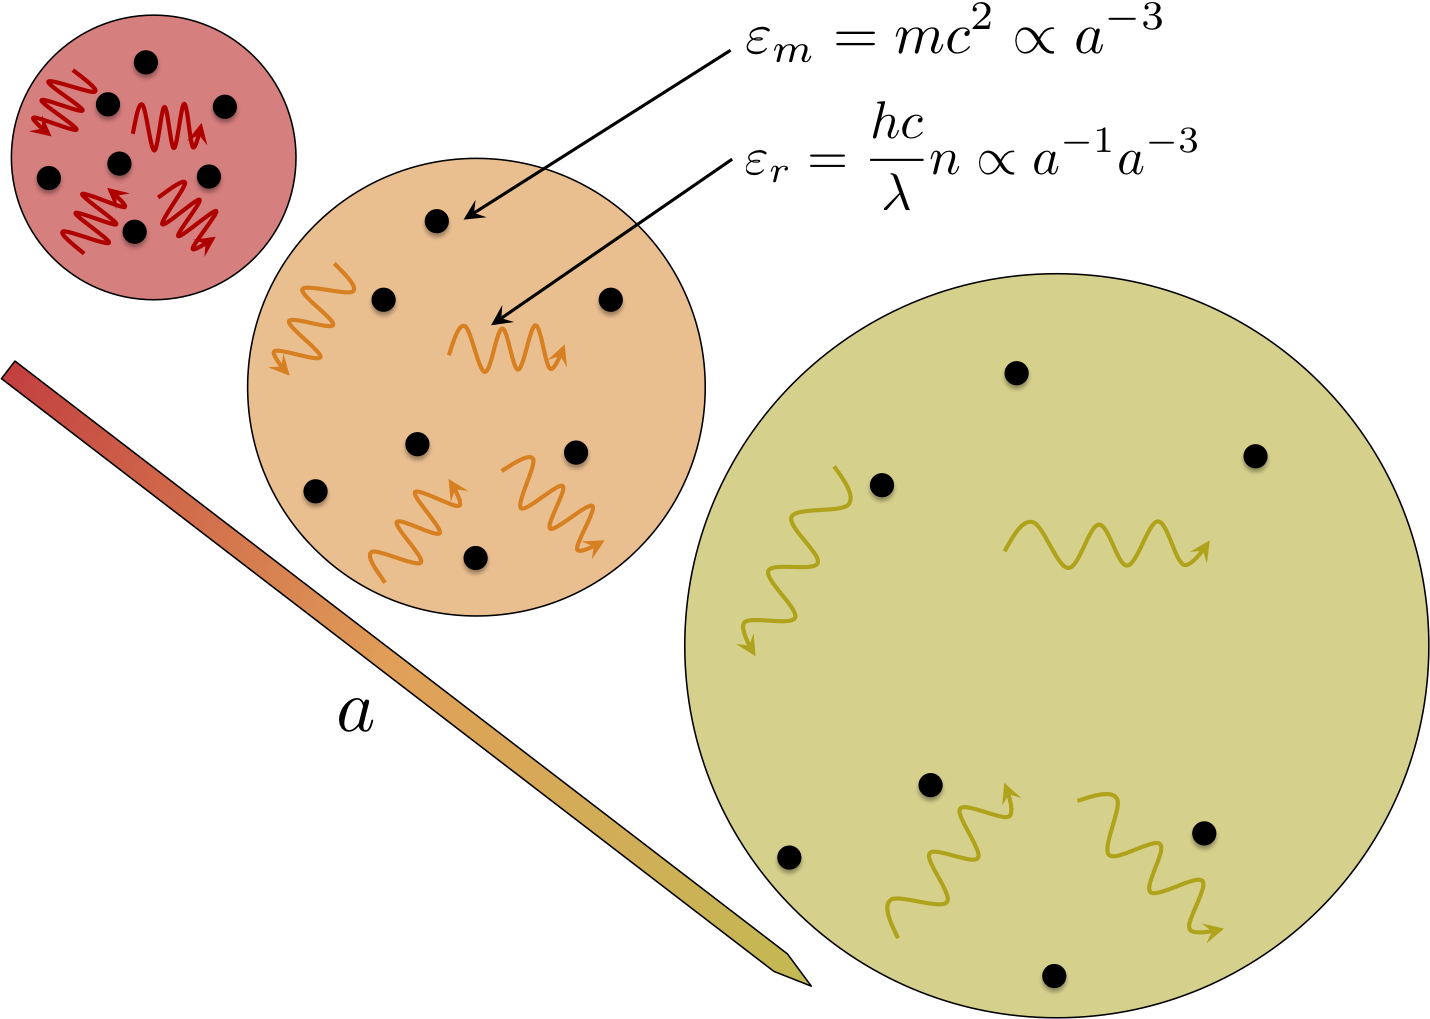
\includegraphics[width=0.75\columnwidth]{Cosmology/mr.png}
\caption{illustration of the evolution of radiation and non-relativistic matter energy density with scale factor. Radiation density decreases as the volume expands, just as for matter, but their associated wavelength gets stretched as well.}
\label{fig:expa}
\end{center}
\end{figure}


For non-relativistic particles, the rest energy dominates over the kinetic term. Notating $v^i = dx^i / dt$ the components of their comoving peculiar velocity, the magnitude of their 3-velocity is $v^2 = a^2 \gamma_{ij} v^i v^j$ and so  \\

\begin{equation}
P^i = m \frac{dt}{ds} v^i = \frac{mv^i}{\sqrt{1-a^2 \gamma_{ij} v^i v^j}} = \frac{m v^i}{\sqrt{1-v^2}}
\end{equation} \\
For relativistic particles on the other hand, the kinetic energy term is preponderant over mass, and so $EdE = pdp$ which yields\\

\begin{equation}
\label{eq:momentum_ur}
\begin{array}{ccc}
\cfrac{\dot{p}}{p} = \cfrac{\dot{a}}{a} = 0 & \Leftrightarrow & p \propto a^{-1}
\end{array}
\end{equation} \\ for relativistic particles. The photon's 4-momentum\footnote{the $\gamma$ index stands for ``photon'', not for a spactime component} $\pmb{P}_\gamma = \left( h \nu / c, -1, -1, -1 \right)$ is proportional to its frequency $\nu = c/\lambda$. It follows from Eq.~\ref{eq:momentum_ur} that a photon's wavelength scales as $a(t)$. Since everything we deduce from the Universe comes from the light emitted by distant luminous objects, this shift in the photon's wavelength red-wards as the Universe expands has to be taken into account as it conceals the expansion rate along its free-falling flight. It is useful to define the quantity $z$ such that \\

\begin{empheq}[box=\mymath]{equation}
\label{def:redshift}
1 + z \doteq \frac{\lambda}{\lambda_0} = \frac{a_0}{a(t)} \geqslant 1
\end{empheq} \\
where $\lambda_0$ is the photon's wavelength in its proper inertial frame at time of emission $t$ and $\lambda$ its wavelength as measured by an observer at time $t_0$ in their frame of reference. Because $a(t) \leqslant a_0 = 1$, $z$ is always positive, meaning the photon's wavelength is always shifted redwards. As such, $z$ is known as the cosmological \textbf{redshift}. It is a purely observational quantity \emph{that does not require a cosmological model}. A photon's wavelength will be redshifted due to 3 main effects:\\
\begin{itemize}
\item[$\bullet$] the Einstein effect, \textit{i.e.} the difference in magnitude of the gravitational field between the observer and the photon's source if the gravitational field is strong;\\
\item[$\bullet$] the Doppler effect, \textit{i.e.} the relative peculiar velocity between the source and the observer; and\\
\item[$\bullet$] the cosmological redshift, which is a pure consequence of the source and the observer being at different coordinates in a \emph{non-inertial} reference frame.\\
\end{itemize}
In this thesis, I study the light coming from very distant luminous objects, quasars, which I introduce in Sec.~\ref{sec:qso}. The light is emitted from a disk region around a supermassive black hole, far from where the Einstein effect can be noticeable. I am working under the assumption that galaxies and quasars are stationary in the comoving coordinate system. The total redshift is thus dominated by the cosmological redshift $z$, and as such I make no distinction between total and cosmological redshift. For objects in the Hubble flow, the cosmological redshift is linear with distance at first order. By expanding the scale factor into an infinite series,\\

\begin{equation}
\label{def:deva}
a(t) = \sum_{k=0}^{\infty} \left( t-t_0 \right)^k \frac{d^k a}{dt^k} (t_0)= a_0 \times \left[ 1 + (t-t_0) \left. \frac{\dot{a}}{a} \right\vert_{t_0} + (t-t_0)^2 \left. \frac{\ddot{a}}{a} \right\vert_{t_0} + \hdots \right]
\end{equation} \\ we can identify the expansion rate as the first order term. The second order term is known as the acceleration parameter, more often rescaled as $\ddot{a} a / \dot{a}^2$. For objects close enough so that $t-t_0$ is negligeable with respect to the conformal age of the Universe,
\begin{equation}
\label{eq:hubble_approx}
z \simeq H_0 \times d
\end{equation} where $d = (t-t_0)$ in units of $c$. The current value of this function $H_0 = H(t_0)$ is often expressed in units of $100~\mathrm{km}~s^{-1}\mathrm{Mpc}^{-1}$ since the significant digits are not quite precice to this day, depending on which data set is used. Commonly, $h \sim 0.7$ within an uncertainty of $\sim 10~\%$, where
\begin{equation}
\label{eq:h}
H(t) = 100~h~\mathrm{km}\cdot s^{-1} \cdot \mathrm{Mpc}^{-1}
\end{equation} Since the scale factor is an undetermined function of time, so is its rate of change. When quoting values for $h$, unless specified otherwise, it is implicitely assumed to be at current time $t_0$. The $0$ subscript is removed for concision purposes as distances and most cosmological parameters are expressed in terms of $h$. The evolution of $a$ and $h$ in time depend mostly on the entropy density of the Universe and thus solving the thermodynamics of the Universe is required at very early times.




\subsection{The Warping of Spacetime}

As previously stated, what is experienced as a gravitational acceleration by an observer is, in general relativity, an inertial acceleration that manisfests due to spacetime curvature. The Newtonian limit is embedded in the so-called Einstein field equations, which quantify the local curvature of spacetime. In this subsection, I detail what is spacetime curvature and what its value is in the FRW metric that describes the Universe's global geometry.  
 
\subsubsection{Spacetime Curvature}

Imagine two travellers starting at the Earth's equator at different longitudes and both heading straight North. Even though they are on parallel trajectories, their paths \emph{will} cross at the North pole. The angles of the triangle their paths form with the segment seperating their starting positions on the equator sum to more than $\pi$ radians. This is due to the non-Euclidian nature of the surface of a spherical Earth. If you've ever wondered why something was missing as you flattened the skin of a ripe clementine after you've peeled it away from the fruit, you were not mistaking: there literally is something missing, preventing you from flattening it into a uniform and uninterupted $\mathbb{R}^2$ plane. The curvature of the spherical surface --- be it the skin of a clementine or the Earth's crust --- is intrinsically linked to the connection of its metric $\pmb{\Gamma}$. The reason our two travellers met on parallel lines is because the covariant derivatives are only comutative in flat space. In general relativity, the 4-dimensional spacetime at a point (event) $P$ is the tangential space at point $P$ of a 5-dimensional \textbf{manifold} $\mathbb{M}$ and is usually written as $\mathcal{T}_P(\mathbb{M})$. In general, given three vectors, $(\vec{u}, \vec{v}, \vec{w}) \in \mathcal{T}^3_P (\mathbb{M})$,
\begin{equation}
\label{def:riemann_curvature_def}
\vec{\nabla}_{\vec{u}} \vec{\nabla}_{\vec{v}}~ \vec{w} = \vec{\nabla}_{\vec{v}} \vec{\nabla}_{\vec{u}} ~\vec{w} + R(\vec{u}, \vec{v})~\vec{w}
\end{equation} where the endomorphism
\begin{eqnarray}
\begin{array}{ccc}
\mathcal{T}_P(\mathbb{M}) & \longrightarrow & \mathcal{T}_P(\mathbb{M})\\
\vec{w} & \longmapsto & R(\vec{u}, \vec{v})~\vec{w}
\end{array}
\end{eqnarray} is linear in $\vec{u}$ and $\vec{v}$ and so defines a tensor, known as the Riemann curvature. It quantifies the non-commutativity of the covariant derivative. Given the following property of the Levi-Civita connection (implicit in $\nabla$): 
\begin{equation}
\label{eq:doublecov}
\nabla^2_{\vec{u}, \vec{v}} = \vec{\nabla}_{\vec{u}} \vec{\nabla}_{\vec{v}}~ \vec{w} - \vec{\nabla}_{\vec{\nabla}_{\vec{u}}\vec{v}} \vec{w}
\end{equation} the Riemann curvature tensor can be identified as
\begin{equation}
\label{def:riemann_curvature}
R(\vec{u}, \vec{v}) = \nabla^2_{\vec{u}, \vec{v}} - \nabla^2_{\vec{v}, \vec{u}}
\end{equation} To illustrate its purpose, Fig.~\ref{fig:parallel_tranport} shows the parallel transport of $\vec{w}$ along $\vec{u}$ and then $\vec{v}$, in comparison to along $\vec{v}$ and then $\vec{u}$. If one starts from the North Pole and keeps pointing South while traveling due South to the equator, then East to a quarter of the circumference of the Earth and then North again to one's starting position, his/her final pointing direction will be $\pi/2$ radians off of its original direction. In Euclidian geometry, the Riemann curvature tensor is zero and transporting $\vec{w}$ along any path will not alter its direction; the covariant derivatives are commutative, and the sum of the angles of a triangle is always $\pi$ radians.\\

\begin{figure}
\begin{center}

\includegraphics[width=0.8\columnwidth]{Cosmology/parallel_transport.png}
\caption{The orange arrows all point ``southwards'', but since the Earth's Riemann curvature isn't null, the parallel transport of the orange vector along meridians and parallels does not conserve direction.}
\label{fig:parallel_tranport}
\end{center}
\end{figure}


The components of the Riemann curvature tensor can be expressed in terms of the Levi-Civita connection defined in Appendix~\ref{apx:covariant}: \\
\begin{equation}
\label{eq:Riemann_Tensor_explicit}
\begin{array}{cl}
R^i_{jk\ell} &\doteq dx^i \left( R(\vec{\partial}_k, \vec{\partial}_\ell) ~\vec{\partial}_j \right)\\
&= \partial_k \Gamma^i_{\ell j} - \partial_\ell \Gamma^i_{k j} + \Gamma^i_{k m} \Gamma^m_{\ell j} - \Gamma^i_{\ell m} \Gamma^m_{k j}\\
&= g^{im} R_{mjk\ell}
\end{array}
\end{equation} \\ The curvature $\mathcal{R}$ of the vector space being considered is simply the trace of the Riemann curvature tensor. For the 2-dimensional surface of the Earth, the curvature \textit{a.k.a.} the Ricci scalar\footnote{because it appears in the Ricci identity} is twice the inverse of its radius squared. For the FRW metric,
\begin{equation}
\label{eq:Ricci_scalar}
\mathcal{R} = g^{\mu \nu} R^{\alpha}_{\mu  \alpha \nu} = - 6 \left( \frac{\ddot{a}}{a} + \left( \frac{\dot{a}}{a} \right)^2 + 2 \frac{\kappa}{a^2} \right)
\end{equation} The Riemann curvature tensor with its first and third indices contracted $R^{\alpha}_{\mu  \alpha \nu} = R_{\mu \nu}$ has the same divergence as the metric tensor $\pmb{g}$ from which it is defined. The Einstein tensor, defined as $\pmb{G} = \pmb{R} - \mathcal{R}/2 ~\pmb{g}$, is thus divergence free. In fact, it is the only rank 2 tensor made from the second derivatives of the metric that features this property, which is useful in establishing the conservation of energy in the framework of general relativity. In order to do so, the warping of spacetime, encapsulated in the Einstein tensor, must be linked to its source and drain terms. In a Universe whose geometry is described by the FRW metric, the non-trivial components of  $G^\mu_\nu = g^{\mu \alpha} G_{\alpha \nu}$ are, using Eq.~\ref{eq:Riemann_Tensor_explicit} and Eq.~\ref{eq:Ricci_scalar} on Eq.~\ref{eq:RWmetric},

\begin{equation}
\label{eq:einsfrw}
\left\{
\begin{array}{l}
G^0_0 = 3 \left[ \left( \cfrac{\dot{a}}{a} \right)^2 + \cfrac{\kappa}{a^2} \right]\\
G^i_j = 2 \left[ \cfrac{\ddot{a}}{a} \left( \cfrac{\dot{a}}{a} \right)^2 + \cfrac{\kappa}{a^2} \right] ~\delta^i_j
\end{array}
\right.
\end{equation}


\subsubsection{Source Terms}

The source terms for the warping of spacetime must come from the local energy content. The rank 2 tensor encapsulating the energy of matter is the stress-energy tensor $\pmb{T}$ whose general covariant expressions of its components are moments of the distribution function \\
\begin{empheq}[box=\mymath]{equation}
\label{eq:nrj_general}
T_{\mu \nu} = \frac{g}{(2 \pi)^3} \int dP_1 dP_2 dP_3 ~\frac{P_\mu P_\nu}{\sqrt{-g} P^0} ~ f(x^i, P_j, \tau)
\end{empheq} \\ where $(-g)^{-1/2} = a^{-4}$ is the metric's trace. The distribution function $f$ is the probability of occupying a given state $(\vec{x}, \vec{P}, t)$ in phase space. The number of particles with $g$ spin states in phase-space volume\footnote{the density of states in a given phase-space is $g/ h^3$ or $g/(2 \pi)^3$ in units of $\hbar = h/2\pi$} $d^3\vec{x} d^3\vec{P} = dx^1 dx^2 dx^3 dP_1 dP_2 dP_3$ is given by \\
\begin{equation}
dN = \frac{g}{(2\pi)^3} ~f(x^i, P_j, \tau)~ d^3\vec{x} d^3\vec{P}
\end{equation} The numerical density of particles is therefore the zeroth moment of the distribution function:
\begin{equation}
\label{eq:number_density}
n(x^i, \tau) = \frac{g}{a^4} \displaystyle \int \frac{d^3P}{(2 \pi)^3} ~f(x^i, P_j, \tau)
\end{equation}

At any given time, the distribution function obeys the Boltzmann equation\\

\begin{empheq}[box=\mymath]{equation}
\mathbb{L}\left[ f \right] = \mathcal{C} \left[ f \right]
\end{empheq} \\ where the Liouville operator $\mathbb{L} \doteq d/ds$ is the derivative along the particle's worldline and the collision functionals $\mathcal{C}$ encapsulate all collision terms and are determined by particle physics.\\

The particle's individual 4-momentum in the FRW metric is
\begin{equation}
\pmb{P} = \left( \epsilon, \vec{q} \right)
\end{equation} with $\vec{q} = q \hat{q} = a \vec{p} = \vec{p}/T$ where $\vec{p}$ is the particle's \emph{proper} momentum as measured by an observer stationary in the comoving coordinate system and $\epsilon(q) = a E = E/T = \sqrt{a^2 m^2 + q^2}$. It is useful to use $\vec{q}$ and $\epsilon$ instead of $\vec{p}$ and $E$ since these quantities are not redshifted, hence we can call them the particle's comoving momentum and comoving energy. We can express the stress energy tensor's components in terms of these quantities, respectively the energy density, the flux of relativistic mass accross the surface normal to $x^i$ and the shear stress tensor:\\

\begin{equation}
\label{sys:stress_energy_tensor_components}
\left\{
\begin{array}{ll}
\rho c^2 = & T^0_0 = -\cfrac{1}{a^4} \displaystyle \int \cfrac{d^3q}{(2\pi)^3}~ \epsilon~ f(\vec{x}, \vec{q}, \tau)\\
\\
\vec{\varphi} c^2 = & T^0_i = \cfrac{1}{a^4} \displaystyle \int \cfrac{d^3q}{(2\pi)^3}~ q_i~ f(\vec{x}, \vec{q}, \tau) = - T_0^i\\
\\
\Sigma^i_j = & T^i_j = \cfrac{1}{a^4} \displaystyle \int \cfrac{d^3q}{(2\pi)^3}~ \cfrac{q^i q_j}{\epsilon}~ f(\vec{x}, \vec{q}, \tau)
\end{array}
\right.
\end{equation} \\

The diagonal elements of the shear stress tensor are known as normal stress \textit{a.k.a.} pressure $\mathcal{P}^i$ exerted on surface normal to $x^i$, while the non-diagonal elements
\begin{equation}
\Sigma^{i,j \neq i} = \sigma^{ij} = \frac{1}{2} \left( \frac{\partial v^j}{\partial x^i} + \frac{\partial v^i}{\partial x^j} \right)
\end{equation} correspond to shear 3-velocity ($\vec{v} = d\vec{x}/dt$) displacement on the surface normal to $x^j$ in the $x^i$ direction, known as anisotropic stress. Because the 4-momentum and 4-velocity are linked via $\pmb{P} = mc~\pmb{u}$, and since pressure is isotropic ($\mathcal{P}^i = \mathcal{P}$), one can write the stress energy tensor in the following tensoral form 
\begin{equation}
\pmb{T} = (\rho + \mathcal{P})~ \pmb{u} \otimes \pmb{u} + \mathcal{P}\pmb{g} + \pmb{\Sigma}
\end{equation} where $\otimes$ denotes the tensoral product.\\

In the spatially homogenous and isotropic background, spatial vectors are vanishing, \textit{i.e.} $\vec{\varphi} c^2 = \vec{0}$ and there is no anisotropic stress, \textit{i.e.} $\pmb{\sigma} = \pmb{0}$, hence the stress energy tensor is diagonal and its contravariant components are

\begin{equation}
\label{eq:stress_fluid}
T^{\mu \nu} = \rho \left[ (w+1) u^\mu u^\nu - w g^{\mu \nu} \right]
\end{equation} which one may recognize as the stress-energy tensor of a perfect fluid of 4-velocity $\pmb{u}$ with an equation of state linking its dynamic pressure $\mathcal{P}$ to the energy density:
\begin{equation}
\label{eq:eos}
\mathcal{P} = w \rho c^2
\end{equation} The perfect fluid approximation is technically \emph{not} valid in the sense that the components of the Universe are not fluids: dark matter for instance does not interact and so cannot define a pressure on its surroundings. However, in absence of anisotropic stress --- which holds true only in the unperturbed background --- the stress energy tensor has the mathematical form of a perfect fluid \emph{a posteriori}. In an abuse of language, we can thus treat the components of the Universe as a perfect fluid at first approximation. The fluid approximation still holds for first order perturbations, which I describe in the next chapter. However, the perturbed cosmological fluid is not perfect as it features anisotropic stress. \\

\subsubsection{From Einstein to Friedmann}

I now postulate (and do not demonstrate !) the Einstein field equations (EFEs), which link the Einstein tensor to the source terms of curvature. They are a set of 10 highly-coupled non-linear second-order differential equations whose solutions are the components of the metric tensor:
\begin{empheq}[box=\mymath]{equation}
\label{eq:EFEs_tensor}
\pmb{G} = \frac{8 \pi G}{c^4} \pmb{T}
%\end{equation}
\end{empheq} with $G$ the universal gravitational (or Newton) constant and the source term $\pmb{T}$ is the stress-energy tensor. \\

These field equations can be used to solve for the internal structure of white dwarfs or neutron stars (where the warping of spacetime is significant and a Newtonian description for the hydrodynamic equilibrium is inadequate), known as the Tolman-Oppenheimer-Volkoff (TOV) equations. In the framework of cosmology, we make use of the Einstein field equations in the opposite way: we postulate from the cosmological principle that the metric is the FRW metric and plug it into the EFEs to extract the conservation laws in the context of an expanding Universe. For the background, the Einstein tensor is diagonal, and so too must be the stress-energy tensor. This gets the number of independant field equations down to 4. Because of homogeneity and isotropy, the 3 spatial ones are redundant and the only 2 independant non-trivial equations are known as the Friedmann equations, using Eq.~\ref{eq:einsfrw}\\

\begin{equation}
\left\{
\begin{array}{lcl}
G^0_0 = 8 \pi G ~T^0_0 & \Rightarrow & \left( \cfrac{\dot{a}}{a} \right)^2 + \cfrac{\kappa}{a^2} - \cfrac{8 \pi G}{3} \rho = 0\\
G^i_j = 8 \pi G ~T^i_j & \Rightarrow & \cfrac{\ddot{a}}{a} + \cfrac{4 \pi G}{3} \left( 1+3w \right) \rho
\end{array}
\right.
\end{equation} \\ These equations are the equivalent of the Poisson and Euler equations of a fluid at rest in a comoving frame of reference. One can also get the continuity equation by either combining both Friedmann equations or using Eq.~\ref{eq:connection_x} on $0 = \pmb{\nabla \cdot G} = \pmb{\nabla \cdot T} = \pmb{\nabla}_\mu T^\mu_0$:
\begin{equation}
\label{eq:continuity}
\dot{\rho} + 3(1+w) H \rho = 0
\end{equation} Integrating Eq.~\ref{eq:continuity} to solve for the energy density $\rho$, 
\begin{equation}
\label{eq:rho}
\rho (t) = \rho (t_0) ~ a^{- 3(1+w)H(t)}
\end{equation} The first Friedmann equation along with the equation of state set the time evolution of the scale factor (heretofor undetermined):
\begin{equation}
a(t) = a_0 \times t^{\frac{2}{3 (1+w)}}
\end{equation} The cosmological perfect fluid considered here is \emph{not} mono-phase. It consists of all known (and unknown) particles. I conventionally adopt a very coarse-grain approach and consider the cosmological fluid as an admixture of two main components:\\
\begin{itemize}
\item[$\bullet$] relativistic matter, \textit{a.k.a.} \textbf{radiation}, which consists of all massless bosons including photons as well as fermions whose $\epsilon \simeq q$; and \\
\item[$\bullet$] non-relativistic matter, or \textbf{matter} for short, which consists of all partices whose $\epsilon \simeq a m$. \\
\end{itemize} To obtain the equations of state of these two main components, thereby explicitely determining the time evolution of the scale factor, we must determine the background temperature $T_\gamma$ from the thermodynamics of the Universe.

\clearpage